\documentclass[aspectratio=169]{beamer}

\usetheme{Madrid}
\usecolortheme{default}

\usepackage{amsmath}
\usepackage{amssymb}
\usepackage{graphicx}
\usepackage{tikz-cd}
\usepackage{tikz}
\usetikzlibrary{calc,positioning}
\usepackage{multicol}

% beamer loads hyperref automatically; set options without re-loading it
\hypersetup{hidelinks}

\title{Digital Signal Processing for Data-Driven Science and Engineering}
\subtitle{Course Outline and Motivation}
\author{}
\date{}

\begin{document}

\begin{frame}
  \titlepage
\end{frame}

\section{Course Outline}
\begin{frame}{Course Outline}
This lecture series covers the foundational techniques of digital signal processing, specifically tailored for data-driven science and engineering.
\begin{itemize}
    \item \textbf{Introduction:} Terminology (Quantization, Sampling), Domains (Time vs. Frequency), Notation.
    \item \textbf{Convolution:} The core operation of linear time-invariant systems.
    \item \textbf{Fourier Method:} Frequency domain analysis.
    \item \textbf{Filtering:} Noise removal and signal isolation.
    \item \textbf{Short-time Fourier Transform (STFT):} Generating Spectrograms.
    \item \textbf{Wavelet Transform:} Generating Scalograms for multi-resolution analysis.
\end{itemize}
\end{frame}

\begin{frame}{Signal processing in a machine learning workflow}
\small
\begin{enumerate}
  \item \textbf{Data acquisition}
  \begin{itemize}
    \item Quantization
    \item Sampling
    \item Analog-to-Digital Conversion (ADC)
  \end{itemize}

  \item \textbf{Preprocessing}
  \begin{itemize}
    \item Noise reduction (denoising)
    \item Windowing
    \item FIR / IIR filter design
    \item Nyquist frequency (aliasing constraints)
  \end{itemize}

  \item \textbf{Feature extraction}
  \begin{itemize}
    \item Fourier transform
    \item Spectrograms (STFT)
    \item Wavelet transform
  \end{itemize}
\end{enumerate}

\vfill
{\footnotesize\itshape Note: this is a rough workflow mapping (not a strict categorization). Many topics overlap and the order depends on the application.}
\end{frame}

\section{Motivation: Why Signal Processing?}
\begin{frame}{Motivation: Why Signal Processing?}
Signal processing is critical for handling real-world data, particularly in domains like healthcare where data is inherently noisy and complex.
\end{frame}

\subsection{Challenges in Health Data}
\begin{frame}{Challenges in Health Data}
Health data scientists encounter diverse data types that require robust processing:
\begin{itemize}
    \item \textbf{Physiological Signals:} Time-series data such as ECG, EEG, EMG, blood pressure, and respiration. These contain complex patterns obscured by noise.
    \item \textbf{Medical Images:} CT, MRI, Ultrasound, and X-rays can be viewed as 2D or 3D signals.
    \item \textbf{Wearable Sensor Data:} Continuous streams from smartwatches (activity, glucose, heart rate, sleep) representing longitudinal time-series data.
    \item \textbf{Electronic Health Records (EHRs):} Time-stamped events (medications, lab results) that function as irregular signals.
\end{itemize}
\end{frame}

\subsection{Improving Machine Learning Models}
\begin{frame}{Improving Machine Learning Models}
Applying signal processing techniques improves downstream machine learning performance:
\begin{itemize}
    \item \textbf{Denoising:} Using filters to remove artifacts leads to cleaner data and more accurate classification.
    \item \textbf{Feature Extraction:} Advanced transforms (like Wavelets or Fourier) reveal hidden features that raw data cannot.
\end{itemize}
\end{frame}

\section{Signal Processing vs. Time Series Analysis}
\begin{frame}{Signal Processing vs. Time Series Analysis}
While both fields deal with sequential data, their approaches and goals differ.

\begin{itemize}
    \item \textbf{Time Series Analysis:}
    \begin{itemize}
        \item \textit{Origin:} Statistics, Econometrics, Business.
        \item \textit{Focus:} Forecasting, trend analysis, seasonality (e.g., stock prices, GDP).
        \item \textit{Data:} Often pre-aggregated; preprocessing is less intensive than in signal processing.
    \end{itemize}
    
    \item \textbf{Signal Processing:}
    \begin{itemize}
        \item \textit{Origin:} Electrical Engineering.
        \item \textit{Focus:} Improving signal transmission, storage, quality, and feature extraction.
        \item \textit{Data:} Works with \textbf{raw} sensor data. Handles higher-dimensional data (images, audio) and requires heavy preprocessing/filtering.
    \end{itemize}
\end{itemize}
\end{frame}

\section{Fundamental Concepts}

\subsection{What is a Signal?}
\begin{frame}{What is a Signal?}
A signal is a description of how one parameter varies in relation to another.
\begin{itemize}
    \item \textbf{Example:} In analog electronics, voltage varying over time.
    \item \textbf{Continuous Signal:} Both the dependent parameter (e.g., voltage) and independent parameter (e.g., time) are continuous.
\end{itemize}

To process signals on a computer, we must convert them from continuous to discrete forms via an Analog-to-Digital Converter (ADC). The process is called digitizing.

\end{frame}


\subsubsection{Sampling}
\begin{frame}{Sampling}
Sampling is the reduction of a continuous-time signal to a discrete-time signal.
\begin{itemize}
    \item It discretizes the \textit{independent} variable (time/space).
    \item \textit{Example:} Converting a continuous sound wave into a sequence of samples taken at fixed intervals.
\end{itemize}

\centering
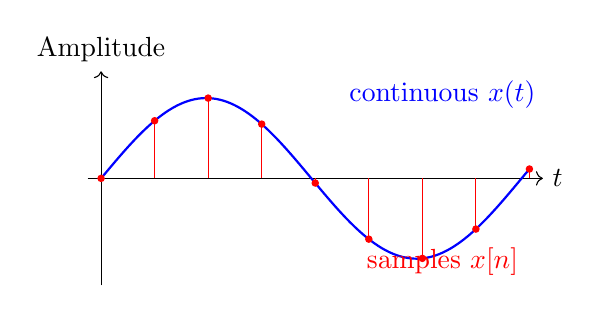
\begin{tikzpicture}[scale=0.85]
  % axes
  \draw[->] (-0.2,0) -- (6.6,0) node[right] {$t$};
  \draw[->] (0,-1.6) -- (0,1.6) node[above] {Amplitude};

  % continuous signal
  \draw[thick,blue,domain=0:6.4,samples=120] plot (\x,{1.2*sin(deg(\x))});
  \node[blue] at (5.1,1.25) {continuous $x(t)$};

  % sampled points + stems
  \foreach \k in {0,0.8,1.6,2.4,3.2,4.0,4.8,5.6,6.4} {
    \fill[red] (\k,{1.2*sin(deg(\k))}) circle (1.6pt);
    \draw[red] (\k,0) -- (\k,{1.2*sin(deg(\k))});
  }
  \node[red] at (5.1,-1.25) {samples $x[n]$};
\end{tikzpicture}

\end{frame}


\subsubsection{Quantization}
\begin{frame}{Quantization}
Quantization is the mapping of input values from a large (continuous) set to a smaller, finite set.
\begin{itemize}
    \item It discretizes the \textit{dependent} variable (amplitude).
    \item Common processes include rounding and truncation.
\end{itemize}

\centering
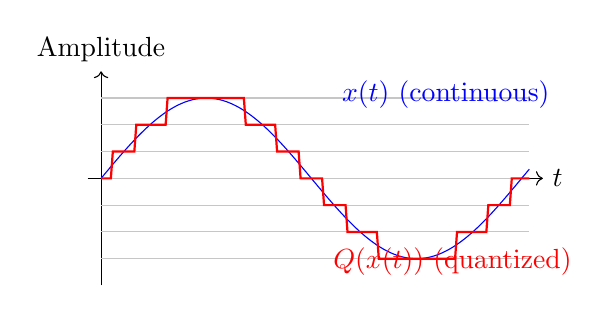
\begin{tikzpicture}[scale=0.85]
  % axes
  \draw[->] (-0.2,0) -- (6.6,0) node[right] {$t$};
  \draw[->] (0,-1.6) -- (0,1.6) node[above] {Amplitude};

  % quantization levels
  \foreach \y in {-1.2,-0.8,-0.4,0,0.4,0.8,1.2} {
    \draw[gray!45] (0,\y) -- (6.4,\y);
  }

  % original continuous signal
  \draw[thin,blue,domain=0:6.4,samples=160] plot (\x,{1.2*sin(deg(\x))});
  \node[blue] at (5.15,1.25) {$x(t)$ (continuous)};

  % quantized output Q(x(t)) over continuous time (no sampling)
  \draw[thick,red,domain=0:6.4,samples=220] plot (\x,{round((1.2*sin(deg(\x)))/0.4)*0.4});
  \node[red] at (5.25,-1.25) {$Q(x(t))$ (quantized)};
\end{tikzpicture}

\end{frame}


\subsubsection{Digitization}
\begin{frame}{Digitization}
\begin{itemize}
    \item \textbf{Discrete/Digitized Signal:} A signal where both time (via sampling) and amplitude (via quantization) are discrete.
\end{itemize}

\centering
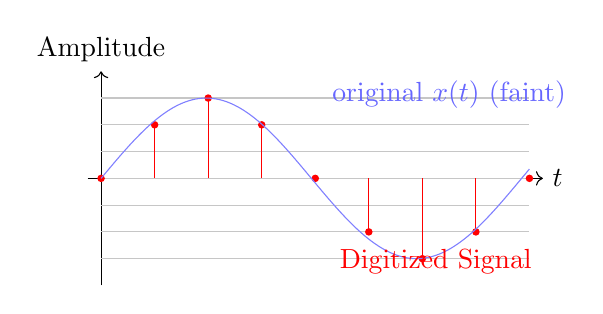
\begin{tikzpicture}[scale=0.85]
  % axes
  \draw[->] (-0.2,0) -- (6.6,0) node[right] {$t$};
  \draw[->] (0,-1.6) -- (0,1.6) node[above] {Amplitude};

  % quantization levels
  \foreach \y in {-1.2,-0.8,-0.4,0,0.4,0.8,1.2} {
    \draw[gray!45] (0,\y) -- (6.4,\y);
  }

  % sampled-and-quantized (nearest level)
  \foreach \k [count=\i from 0] in {0,0.8,1.6,2.4,3.2,4.0,4.8,5.6,6.4} {
    \pgfmathsetmacro{\val}{1.2*sin(deg(\k))}
    \pgfmathsetmacro{\qval}{round((\val)/0.4)*0.4}
    \fill[red] (\k,\qval) circle (1.6pt);
    \draw[red] (\k,0) -- (\k,\qval);
  }

  % show a reference continuous curve faintly
  \draw[thin,blue!50,domain=0:6.4,samples=120] plot (\x,{1.2*sin(deg(\x))});
  \node[blue!60] at (5.2,1.25) {original $x(t)$ (faint)};
  \node[red] at (5.0,-1.25) {Digitized Signal};
\end{tikzpicture}

\end{frame}



\section{Recommended Resources}

\subsection{Theory}
\begin{frame}{Recommended Resources (Theory)}
\begin{itemize}
    \item \textit{The Scientist and Engineer's Guide to Digital Signal Processing}, Steven W. Smith (1999). (Ch 1, 2, 3, 8, 9, 10)
    \item \textit{Data-Driven Science and Engineering}, Steven L. Brunton \& J. Nathan Kutz. (Ch 2 for Fourier, Wavelet)
    \item \textit{Discrete-Time Signal Processing}, Alan V. Oppenheim \& Ronald W. Schafer.
    \item \href{https://eng.libretexts.org/Bookshelves/Electrical_Engineering/Signal_Processing_and_Modeling/Signals_and_Systems_(Baraniuk_et_al.)}{LibreTexts: Signals and Systems}
    \item \href{https://ocw.mit.edu/courses/6-003-signals-and-systems-fall-2011/}{MIT OpenCourseWare: Signals and Systems}
\end{itemize}

Code \& Implementation

\begin{itemize}
    \item \href{https://mwickert.github.io/scikit-dsp-comm/}{Scikit-DSP-Comm}
    \item \href{https://ataspinar.com/2018/12/21/a-guide-for-using-the-wavelet-transform-in-machine-learning/}{Guide to Wavelet Transform in ML}
    \item \href{https://www.kaggle.com/code/faressayah/signal-processing-with-python}{Signal Processing with Python (Kaggle)}
\end{itemize}
\end{frame}


\section{Introduction: Terminology}

\begin{frame}{Domains: time, frequency, spatial}
\small
\begin{itemize}
  \item \textbf{Time domain:} signal as a function of time, $x(t)$ (continuous) or $x[n]$ (discrete).
  \item \textbf{Frequency domain:} spectrum showing how energy is distributed over frequency, $X(f)$ or $X[k]$.
  \item \textbf{Spatial domain:} signal as a function of position (1D/2D/3D), e.g., image intensity $I(x,y)$ or volume $V(x,y,z)$.
  \item \textbf{Same information, different view:} transforms (Fourier / wavelet) map between domains.
\end{itemize}

\vspace{0.5em}
\begin{columns}[T,onlytextwidth]
  \column{0.5\textwidth}
  \centering
  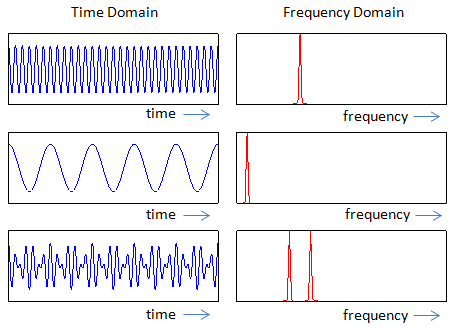
\includegraphics[width=\linewidth,height=0.4\textheight,keepaspectratio]{Figures/timefreq.png}


  \column{0.5\textwidth}
  \centering
  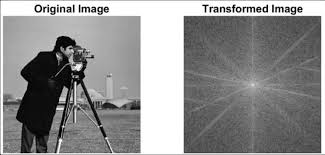
\includegraphics[width=\linewidth,height=0.4\textheight,keepaspectratio]{Figures/spafreq.jpg}


\end{columns}

\end{frame}

\begin{frame}{Domains: time, frequency, spatial}


\begin{columns}[T,onlytextwidth]
  \column{1\textwidth}
  \centering
  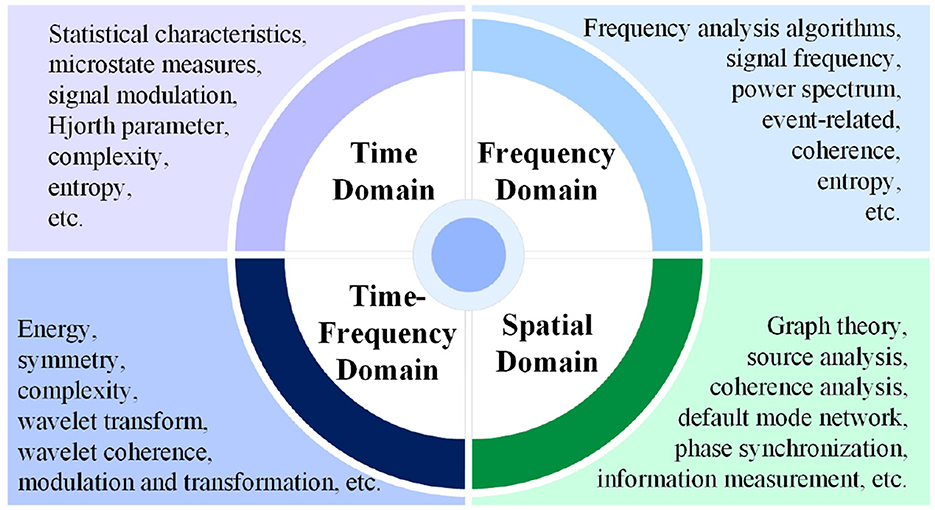
\includegraphics[width=\linewidth,height=0.7\textheight,keepaspectratio]{Figures/timefreqspa.jpg}
\end{columns}


\vfill
{\tiny\raggedright https://www.frontiersin.org/journals/aging-neuroscience/articles/10.3389/fnagi.2025.1686628/full}


\end{frame}

\begin{frame}{Common notation (signals \& indices)}
\small
\begin{columns}[T,onlytextwidth]
\column{0.52\textwidth}
\begin{itemize}
  \item Continuous-time: $x(t)$
  \item Discrete-time: $x[n]$ where $n\in\mathbb{Z}$
  \item Sampling period / rate: $T_s$, $f_s=\tfrac{1}{T_s}$
  \item Complex unit: $j=\sqrt{-1}$ (engineering) or $i$
  \item Fourier transform: $X(f)=\mathcal{F}\{x(t)\}$

\end{itemize}
\column{0.48\textwidth}
\begin{block}{Quick interpretation}
\begin{itemize}
  \item $t$ \textit{continuous} vs. $n$ \textit{integer index}
  \item $f$ in Hz (or $\omega=2\pi f$ in rad/s)
  \item $k$ is a frequency-bin index for an $N$-point DFT
\end{itemize}
\end{block}
\end{columns}
\end{frame}


% -------------------------------------------------
% Expanded content for graduate Data Science (Healthcare)
% -------------------------------------------------


\subsection{Basic signal operations}

\begin{frame}{Basic signal operations: time shift}
\small
\textbf{Continuous-time:} if $y(t)=x(t-t_0)$ then $y$ is $x$ shifted \textbf{right} by $t_0$.

\vspace{0.5em}
\textbf{Discrete-time:} if $y[n]=x[n-n_0]$ then $y$ is $x$ shifted \textbf{right} by $n_0$ samples.

\vspace{0.5em}
\centering
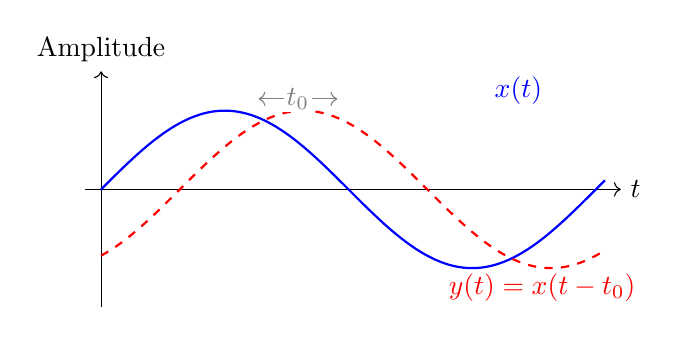
\begin{tikzpicture}[scale=1]
  % axes
  \draw[->] (-0.2,0) -- (6.6,0) node[right] {$t$};
  \draw[->] (0,-1.5) -- (0,1.5) node[above] {Amplitude};

  % original and shifted signals
  \draw[thick,blue,domain=0:6.4,samples=140] plot (\x,{sin(deg(\x))});
  \draw[thick,red,dashed,domain=0:6.4,samples=140] plot (\x,{sin(deg(\x-1.0))});

  % indicate shift t0
  \draw[<->,gray] (2,1.15) -- (3,1.15) node[midway,fill=white,inner sep=1pt] {$t_0$};

  \node[blue] at (5.3,1.25) {$x(t)$};
  \node[red] at (5.6,-1.25) {$y(t)=x(t-t_0)$};
\end{tikzpicture}


\end{frame}

\begin{frame}{Basic signal operations: time scaling}
\small
\textbf{Continuous-time scaling:} $y(t)=x(at)$
\begin{itemize}
  \item $|a|>1$: time \textbf{compression} (faster).
  \item $0<|a|<1$: time \textbf{expansion} (slower).
  \item $a<0$: time reversal.
\end{itemize}

\vspace{0.25em}
\centering
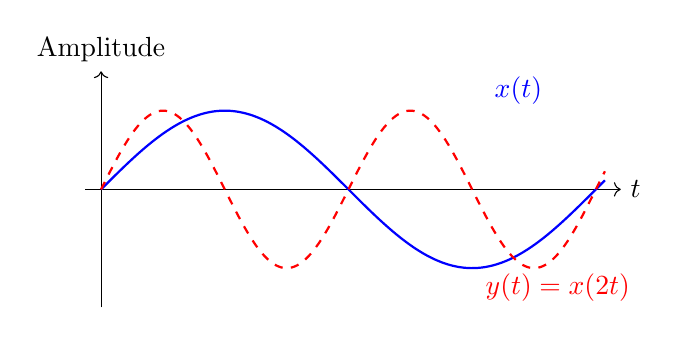
\begin{tikzpicture}[scale=1]
  % axes
  \draw[->] (-0.2,0) -- (6.6,0) node[right] {$t$};
  \draw[->] (0,-1.5) -- (0,1.5) node[above] {Amplitude};

  % original and scaled signals (a=2)
  \draw[thick,blue,domain=0:6.4,samples=140] plot (\x,{sin(deg(\x))});
  \draw[thick,red,dashed,domain=0:6.4,samples=220] plot (\x,{sin(deg(2*\x))});

  \node[blue] at (5.3,1.25) {$x(t)$};
  \node[red] at (5.8,-1.25) {$y(t)=x(2t)$};
\end{tikzpicture}


\end{frame}

\subsection{A system}

\begin{frame}{A system: mapping input to output}
\small
\begin{columns}[T,onlytextwidth]
  \column{0.56\textwidth}
  A \textbf{system} transforms an input signal $x$ into an output $y$:
  \[
   y = \mathcal{T}\{x\}
  \]
  Examples:
  \begin{itemize}
    \item Moving-average smoother (reduces high-frequency noise).
    \item Differentiator (emphasizes rapid changes).
    \item Bandpass filter (isolates frequency bands, e.g., QRS complexes in ECG).
  \end{itemize}

  \column{0.44\textwidth}
  \centering
  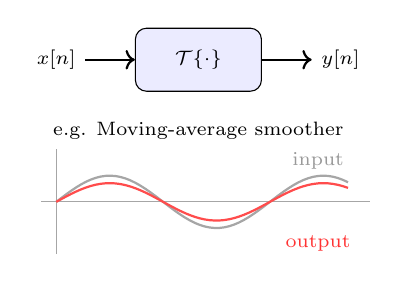
\begin{tikzpicture}[scale=0.95, every node/.style={font=\scriptsize}]
    % input / output nodes
    \node (x) at (0,0) {$x[n]$};
    \node[draw,rounded corners,minimum width=1.6cm,minimum height=0.8cm,fill=blue!8] (T) at (1.9,0) {$\mathcal{T}\{\cdot\}$};
    \node (y) at (3.8,0) {$y[n]$};
    \draw[->,thick] (x) -- (T);
    \draw[->,thick] (T) -- (y);

    % annotate examples
    \node[align=center] at (1.9,-0.95) {e.g. Moving-average smoother};

    % tiny waveform sketch
    \draw[gray!70] (-0.2,-1.9) -- (4.2,-1.9);
    \draw[gray!70] (0,-2.6) -- (0,-1.2);
    \draw[thick,gray!70,domain=0:3.9,samples=60] plot (\x,{-1.9+0.35*sin(deg(2.2*\x))});
    \draw[thick,red!70,domain=0:3.9,samples=60] plot (\x,{-1.9+0.25*sin(deg(2.2*\x))});
    \node[gray!80] at (3.5,-1.35) {input};
    \node[red!80] at (3.5,-2.45) {output};
  \end{tikzpicture}
\end{columns}
\end{frame}

\begin{frame}{System classification}
\small

For a system $y=\mathcal{T}\{x\}$:
\begin{itemize}
  \item \textbf{Linearity:}
  \[
    \mathcal{T}\{a x_1 + b x_2\}=a\,\mathcal{T}\{x_1\}+b\,\mathcal{T}\{x_2\}.
  \]

  \item \textbf{Time invariance:} if $y(\cdot)=\mathcal{T}\{x(\cdot)\}$ then, for any shift $t_0$,
  \[
    \mathcal{T}\{x(\cdot-t_0)\}=y(\cdot-t_0).
  \]

  \item \textbf{Causality:} for every $t_0$, $y(t_0)$ depends only on $\{x(t):t\le t_0\}$.


  \item \textbf{Stability (BIBO):}
  \[
    |x(t)|\le B_x\ \forall t\quad\Rightarrow\quad |y(t)|\le B_y\ \forall t.
  \]

  \item \textbf{Memoryless vs. with memory:}
  \begin{itemize}
    \item Memoryless: $y(t)=f(x(t))$ (depends only on the current input).
    \item With memory: $y(t_0)$ depends on $x(t)$ for some $t\neq t_0$.
  \end{itemize}
\end{itemize}

\end{frame}






\begin{frame}[plain]
    \centering
    \vfill
    {\usebeamerfont{section title}Convolution and Impulse response \par}
    \vfill
  \end{frame}

\subsection{Convolution and cross correlation}

\begin{frame}{Convolution vs. cross-correlation (big picture)}
\small

\begin{columns}[T,onlytextwidth]
  \column{0.55\textwidth}


  \textbf{Convolution (system view)}
  \[
    y[n] = (x*h)[n] = \sum_{k=-\infty}^{\infty} x[k]\,h[n-k]
  \]
  \emph{``Given an LTI system with impulse response $h[n]$, what output do we get for input $x[n]$?''}

  \vspace{0.1em}
  \textbf{Cross-correlation (similarity view)}
  \[
    r_{xy}[\ell] = \sum_{n=-\infty}^{\infty} x[n] \, y[n+\ell]
  \]
  \item \textbf{Cross-correlation:} \emph{``How similar are two signals if one is shifted by $\ell$?''}


  \column{0.45\textwidth}
    \centering
    % Replace this filename with your figure
    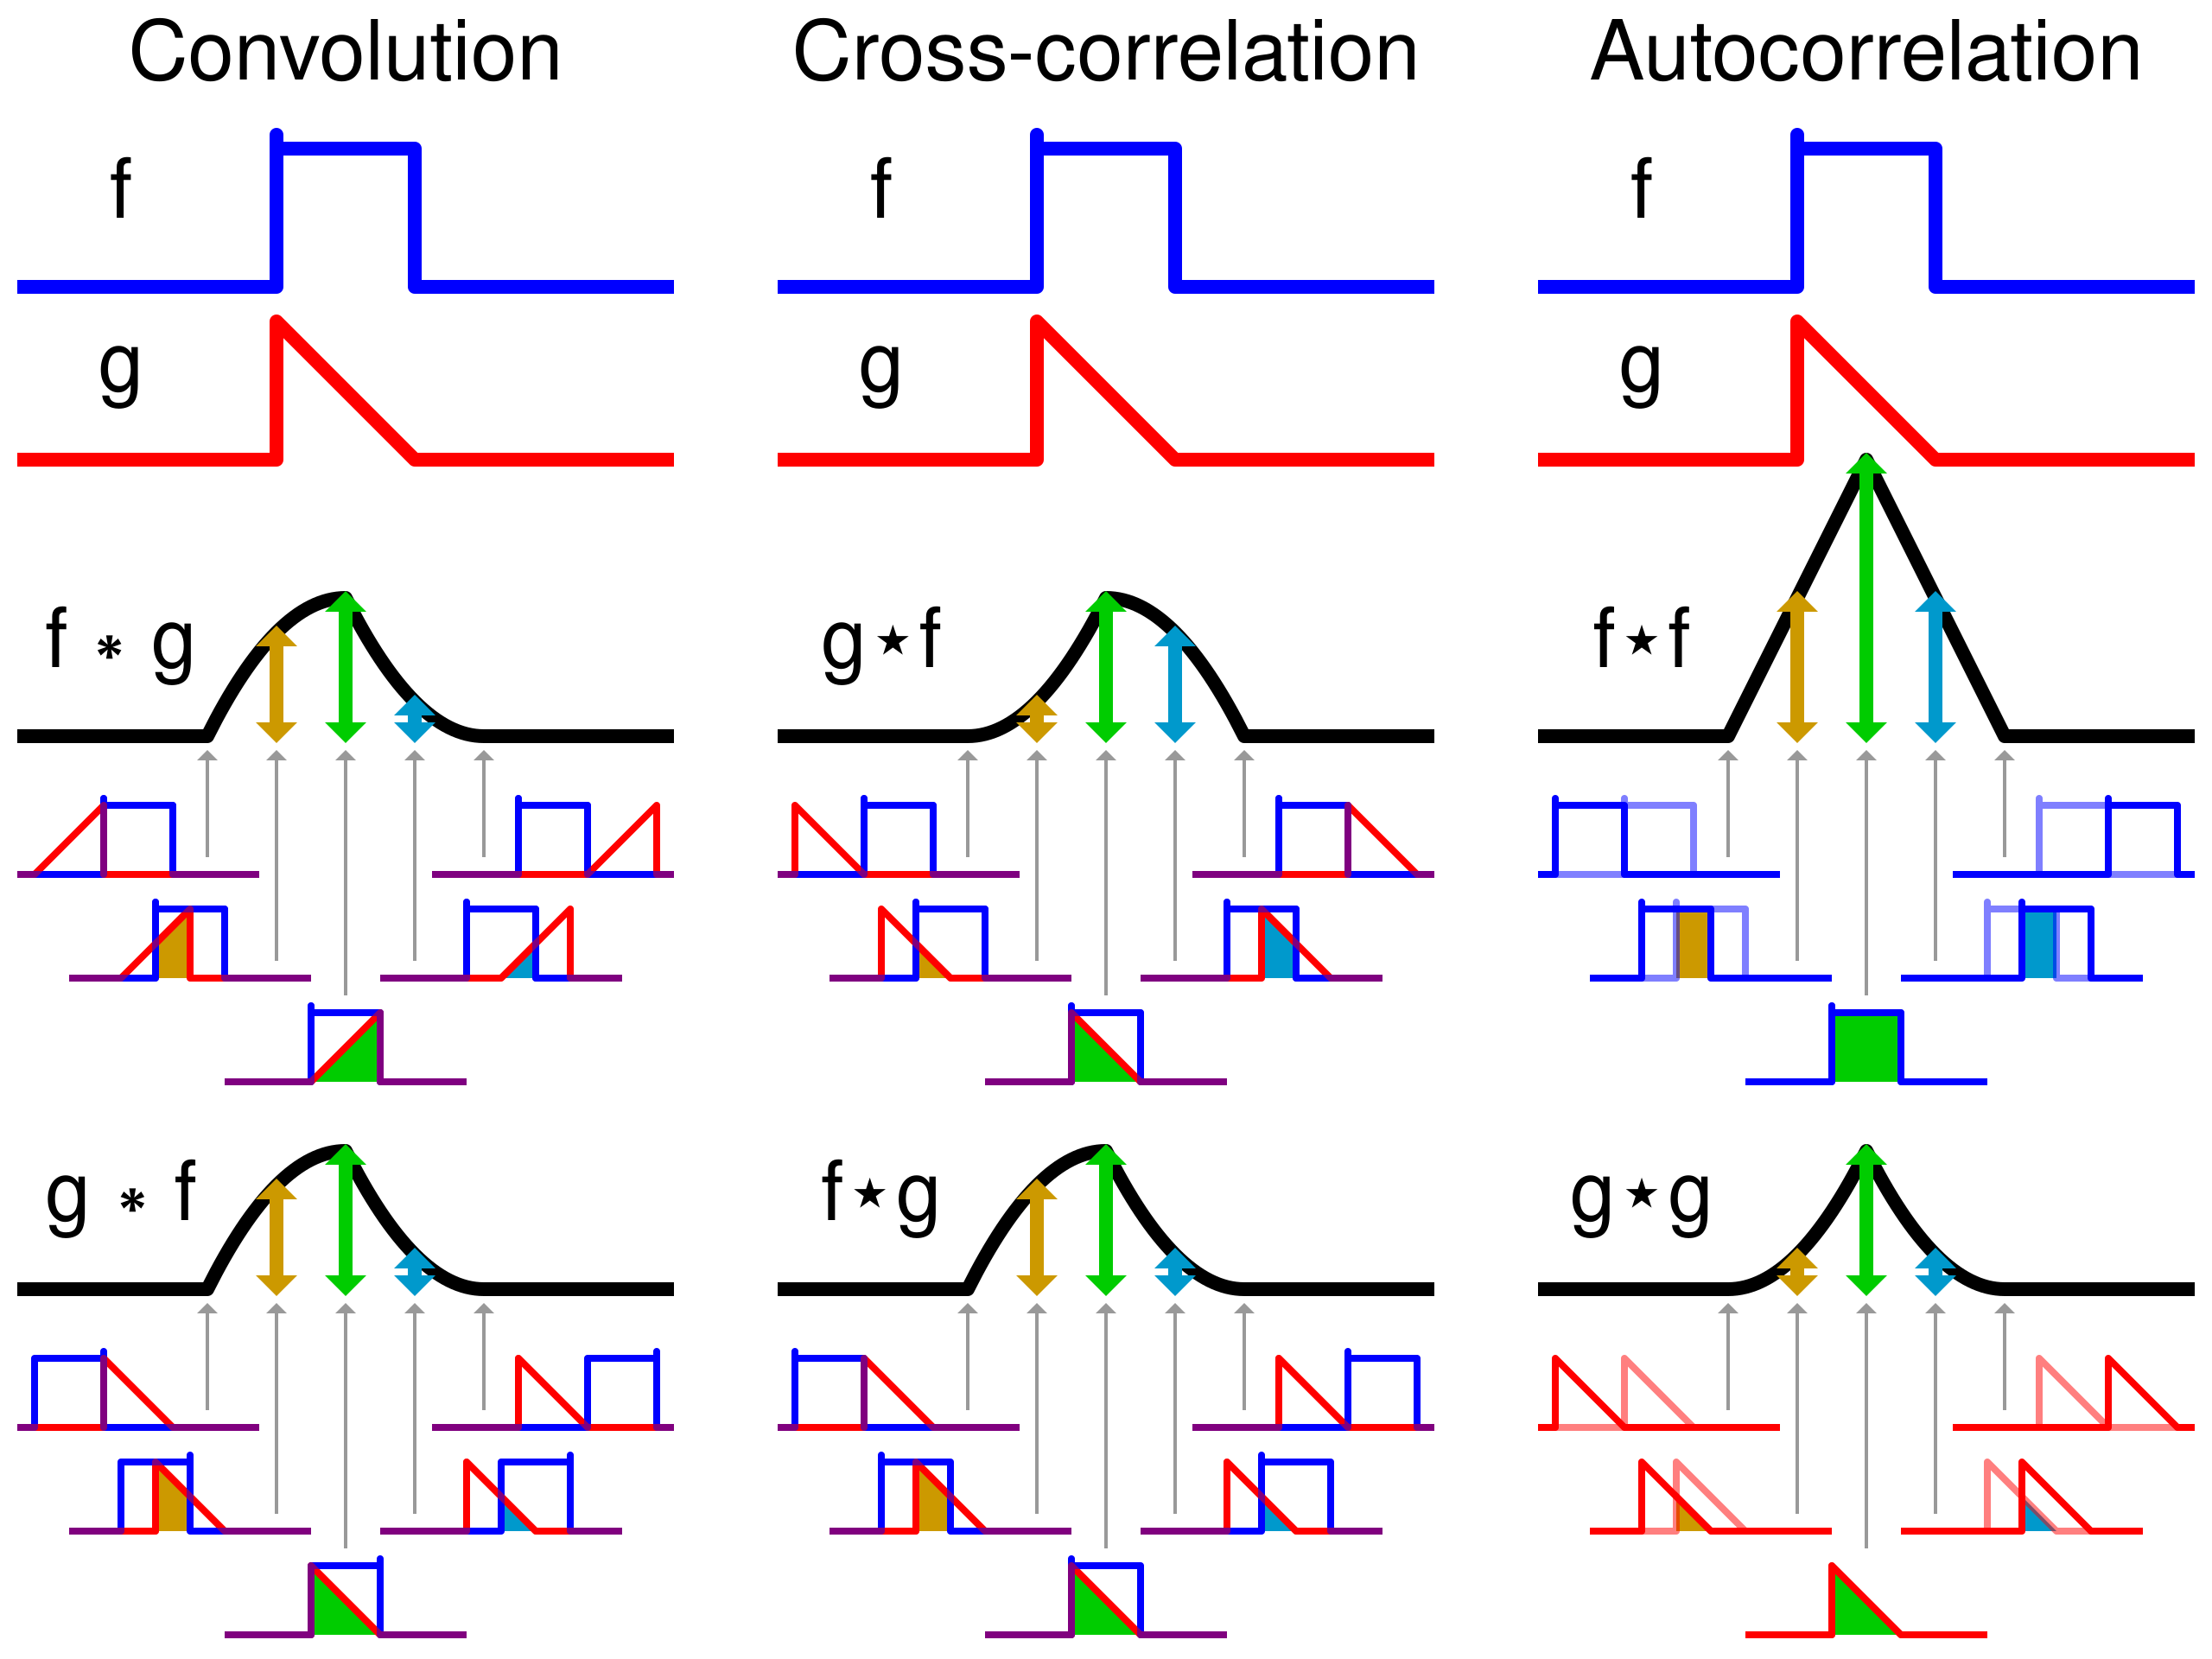
\includegraphics[width=\linewidth,height=0.55\textheight,keepaspectratio]{Figures/corr.png}

\end{columns}
\vspace{-0.1em}
  {\footnotesize\textbf{Interactive demos:} \texttt{youtube.com/watch?v=C1N55M1VD2o} \;|\; \texttt{github.com/phiresky/convolution-demo}}
\end{frame}

\begin{frame}{Convolution: hand-calculation example}
\small
\begin{columns}[T,onlytextwidth]
  \column{0.58\textwidth}
  Let
  \[
    x[n]=\{1,\,2,\,1\}\quad (n=0,1,2),\qquad
    h[n]=\{1,\,1\}\quad (n=0,1).
  \]
  Compute $y[n]=(x*h)[n]=\sum_k x[k]h[n-k]$.

  \vspace{0.3em}
  \begin{align*}
    y[0] &= x[0]h[0] = 1\cdot 1 = 1\\
    y[1] &= x[0]h[1] + x[1]h[0] = 1\cdot 1 + 2\cdot 1 = 3\\
    y[2] &= x[1]h[1] + x[2]h[0] = 2\cdot 1 + 1\cdot 1 = 3\\
    y[3] &= x[2]h[1] = 1\cdot 1 = 1
  \end{align*}

  \vspace{-0.2em}
  So the output is
  \[
    y[n]=\{1,\,3,\,3,\,1\}\quad (n=0,1,2,3).
  \]

  \column{0.42\textwidth}
  \centering
  \vspace{-0.6em}
  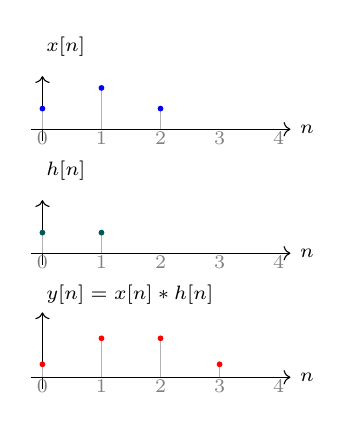
\begin{tikzpicture}[scale=0.75, every node/.style={font=\scriptsize}]
    % helper: axes + stems (simple, fixed ranges)

    % ---- x[n]
    \begin{scope}
      \node[anchor=west] at (-0.1,3.1) {$x[n]$};
      \draw[->] (-0.2,1.7) -- (4.2,1.7) node[right] {$n$};
      \draw[->] (0,1.5) -- (0,2.6);
      \foreach \k/\v in {0/1,1/2,2/1} {
        \draw[gray!60] (\k,1.7) -- (\k,{1.7+0.35*\v});
        \fill[blue] (\k,{1.7+0.35*\v}) circle (1.4pt);
      }
      \foreach \k in {0,1,2,3,4} {\node[gray] at (\k,1.55) {\k};}
    \end{scope}

    % ---- h[n]
    \begin{scope}[yshift=-2.1cm]
      \node[anchor=west] at (-0.1,3.1) {$h[n]$};
      \draw[->] (-0.2,1.7) -- (4.2,1.7) node[right] {$n$};
      \draw[->] (0,1.5) -- (0,2.6);
      \foreach \k/\v in {0/1,1/1} {
        \draw[gray!60] (\k,1.7) -- (\k,{1.7+0.35*\v});
        \fill[teal!70!black] (\k,{1.7+0.35*\v}) circle (1.4pt);
      }
      \foreach \k in {0,1,2,3,4} {\node[gray] at (\k,1.55) {\k};}
    \end{scope}

    % ---- y[n]
    \begin{scope}[yshift=-4.2cm]
      \node[anchor=west] at (-0.1,3.1) {$y[n]=x[n]*h[n]$};
      \draw[->] (-0.2,1.7) -- (4.2,1.7) node[right] {$n$};
      \draw[->] (0,1.5) -- (0,2.8);
      \foreach \k/\v in {0/1,1/3,2/3,3/1} {
        \draw[gray!60] (\k,1.7) -- (\k,{1.7+0.22*\v});
        \fill[red] (\k,{1.7+0.22*\v}) circle (1.4pt);
      }
      \foreach \k in {0,1,2,3,4} {\node[gray] at (\k,1.55) {\k};}
    \end{scope}
  \end{tikzpicture}
\end{columns}
\end{frame}


\subsection{Dirac delta function (unit impulse)}

\begin{frame}{Dirac delta / unit impulse: continuous-time}
\small
The Dirac delta $\delta(t)$ is not a usual function, but it satisfies:
\begin{itemize}
  \item $\delta(t)=0$ for $t\neq 0$ and $\int_{-\infty}^{\infty}\delta(t)\,dt = 1$.
  \item \textbf{Sifting:} $\int_{-\infty}^{\infty} x(t)\,\delta(t-t_0)\,dt = x(t_0)$.
\end{itemize}
\begin{block}{Interpretation}
A delta ``picks out'' the value of a signal at a time point; it is the mathematical model of an ideal impulse.
\end{block}

\centering
\begin{tikzpicture}[scale=0.9]
  % axes
  \draw[->] (-0.2,0) -- (6.4,0) node[right] {$t$};
  \draw[->] (0,-0.2) -- (0,2.0) node[above] {$\delta(t)$};

  % impulse at t0
  \def\tzero{3.2}
  \draw[thick,red,->] (\tzero,0) -- (\tzero,1.6);
  \node[red,above] at (\tzero,1.6) {$1$};
  \node[below] at (\tzero,0) {$t_0$};

  % baseline label
  \node[gray] at (5.6,1.3) {idealized impulse};
\end{tikzpicture}

\end{frame}

\begin{frame}{Unit impulse: discrete-time}
\small
The discrete-time unit impulse is
\[
\delta[n] = \begin{cases}
1, & n=0\\
0, & n\neq 0
\end{cases}
\]
Key identities:
\begin{itemize}
  \item \textbf{Shifting:} $x[n-n_0] = \sum_k x[k]\,\delta[n-n_0-k]$.
  \item \textbf{Sifting:} $\sum_n x[n] \delta[n-n_0] = x[n_0]$.
\end{itemize}

\centering
\begin{tikzpicture}[scale=0.85]
  % axes
  \draw[->] (-3.4,0) -- (3.4,0) node[right] {$n$};
  \draw[->] (0,-0.2) -- (0,1.9) node[above] {$\delta[n]$};

  % stems
  \foreach \k in {-3,-2,-1,0,1,2,3} {
    \draw[gray!55] (\k,0) -- (\k,{(\k==0) ? 1.4 : 0});
    \fill[red] (\k,{(\k==0) ? 1.4 : 0}) circle (1.6pt);
  }
  \node[red,above] at (0,1.4) {$1$};
\end{tikzpicture}

\end{frame}

\begin{frame}{Impulse properties you will use constantly}
\small
\begin{columns}[T,onlytextwidth]
  \column{0.58\textwidth}
  \begin{itemize}
    \item $x[n]*\delta[n]=x[n]$ (identity).
    \item $x[n]*\delta[n-n_0]=x[n-n_0]$ (shift via convolution).
    \item If $h[n]$ is an LTI system response to $\delta[n]$, then $h[n]$ \textbf{fully characterizes} the system.
  \end{itemize}

  \vspace{0.4em}
  \begin{block}{Why this matters}
  It lets us build any input from shifted impulses, then use linearity/time-invariance to predict the output.
  \end{block}

  \column{0.42\textwidth}
  \centering
  \vspace{-0.3em}
  {\footnotesize Example: $x[n]*\delta[n-2]=x[n-2]$ (shift right by 2)}

  \vspace{0.2em}
  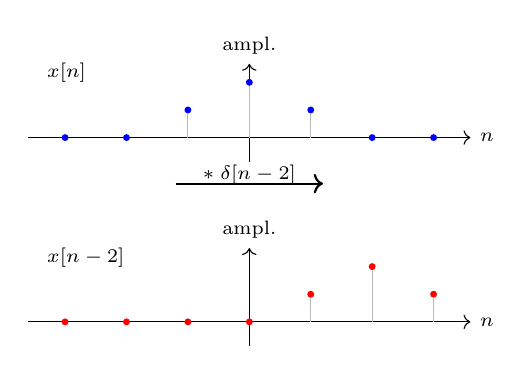
\begin{tikzpicture}[scale=0.78, every node/.style={font=\scriptsize}]
    % ---- top: x[n]
    \begin{scope}
      \draw[->] (-3.6,1.6) -- (3.6,1.6) node[right] {$n$};
      \draw[->] (0,1.2) -- (0,2.8) node[above] {ampl.};
      \node[anchor=west] at (-3.45,2.65) {$x[n]$};

      \foreach \k/\v in {-3/0,-2/0,-1/1,0/2,1/1,2/0,3/0} {
        \draw[gray!55] (\k,1.6) -- (\k,{1.6+0.45*\v});
        \fill[blue] (\k,{1.6+0.45*\v}) circle (1.6pt);
      }
    \end{scope}

    % ---- arrow / operator
    \node at (0,1.0) {$*\;\delta[n-2]$};
    \draw[->,thick] (-1.2,0.85) -- (1.2,0.85);

    % ---- bottom: shifted x[n-2]
    \begin{scope}[yshift=-3cm]
      \draw[->] (-3.6,1.6) -- (3.6,1.6) node[right] {$n$};
      \draw[->] (0,1.2) -- (0,2.8) node[above] {ampl.};
      \node[anchor=west] at (-3.45,2.65) {$x[n-2]$};

      % original nonzeros at n=-1,0,1 -> shift right by 2 -> n=1,2,3
      \foreach \k/\v in {-3/0,-2/0,-1/0,0/0,1/1,2/2,3/1} {
        \draw[gray!55] (\k,1.6) -- (\k,{1.6+0.45*\v});
        \fill[red] (\k,{1.6+0.45*\v}) circle (1.6pt);
      }
    \end{scope}
  \end{tikzpicture}
\end{columns}
\end{frame}

\subsection{Impulse response}

\begin{frame}{Impulse response: definition}
\small
For an LTI system $\mathcal{T}$, the \textbf{impulse response} is
\[
 h[n] = \mathcal{T}\{\delta[n]\}
\]
and the input--output relationship is
\[
 y[n] = x[n] * h[n].
\]
\begin{block}{Equivalent viewpoint}
Filtering is ``pattern matching'' between the input and the impulse response shape.
\end{block}
\end{frame}

\begin{frame}{Why impulse response is important (Applications)}
\small
\begin{itemize}
  \item Determines \textbf{what gets smoothed or amplified} (noise vs. signal).
  \item FIR filtering (choose $h[n]$ directly; stable and interpretable).
  \item IIR filtering (recursive; efficient but needs stability checks).
  \item Feature engineering for ML (energy in bands, envelope extraction, derivatives).
\end{itemize}
\begin{block}{Healthcare examples}
\begin{itemize}
  \item Low-pass $h[n]$ for motion artifact reduction in PPG.
  \item Band-pass $h[n]$ to isolate rhythms in ECG/EEG.
  \item Deconvolution https://www.youtube.com/watch?v=yNOPIVnsot8
  \item Visual microphone https://www.youtube.com/watch?v=FKXOucXB4a8
\end{itemize}
\end{block}
\end{frame}




\begin{frame}{Why use block diagrams?}
\small
Block diagrams give a compact picture of a system's \textbf{computational structure}.
\begin{itemize}
  \item Show \textbf{signal flow} and interconnections between stages.
  \item Enable \textbf{modular analysis/design} (break complex systems into simple blocks).
  \item Make LTI systems (e.g., difference equations) easier to \textbf{implement, debug, and communicate}.
\end{itemize}
\end{frame}

\begin{frame}{Common block-diagram elements}
\small
\centering
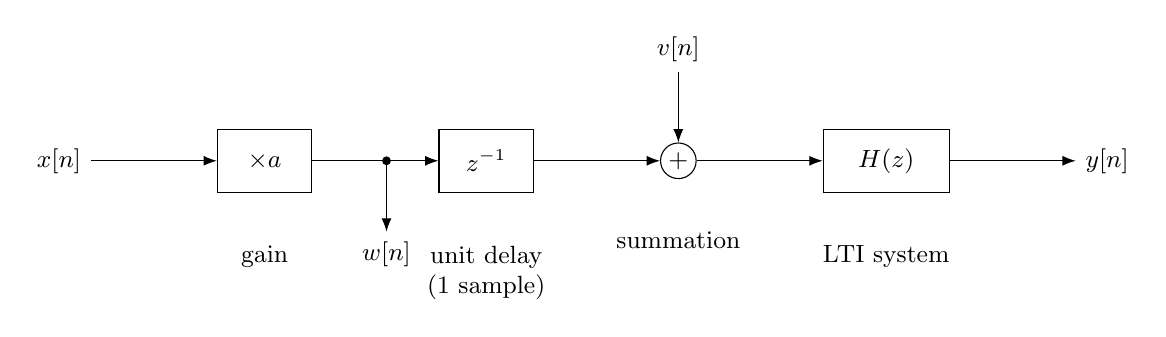
\begin{tikzpicture}[
  node distance=1.6cm,
  >=Latex,
  every node/.style={font=\small}
]

  % main signal path
  \node (x) {$x[n]$};
  \node[draw,minimum width=1.2cm,minimum height=0.8cm,right=of x] (gain) {$\times a$};
  \node[draw,minimum width=1.2cm,minimum height=0.8cm,right=of gain] (delay) {$z^{-1}$};
  \node[circle,draw,inner sep=1.2pt,right=of delay] (sum) {$+$};
  \node[draw,minimum width=1.6cm,minimum height=0.8cm,right=of sum] (sys) {$H(z)$};
  \node[right=of sys] (y) {$y[n]$};

  \draw[->] (x) -- (gain);
  \draw[->] (gain) -- (delay);
  \draw[->] (delay) -- (sum);
  \draw[->] (sum) -- (sys);
  \draw[->] (sys) -- (y);

  % second input into summer
  \node[above=0.9cm of sum] (v) {$v[n]$};
  \draw[->] (v) -- (sum);

  % branch / tap example
  \coordinate (tap) at ($(gain)!0.55!(delay)$);
  \fill (tap) circle (1.6pt);
  \node[below=0.9cm of tap] (w) {$w[n]$};
  \draw[->] (tap) -- (w);

  % labels under elements
  \node[below=0.55cm of gain,align=center] {gain};
  \node[below=0.55cm of delay,align=center] {unit delay\\(1 sample)};
  \node[below=0.55cm of sum,align=center] {summation};
  \node[below=0.55cm of sys,align=center] {LTI system};

\end{tikzpicture}

\vspace{0.6em}
\begin{itemize}
  \item \textbf{Gain:} $y[n]=a\,x[n]$ 
  \item \textbf{Delay:} $y[n]=x[n-1]$
  \item \textbf{Summation:} $y[n]=x_1[n]+x_2[n]$  
  \item \textbf{Branch:} copies a signal to multiple paths
  \item \textbf{System block:} an operator (e.g., filter) mapping input to output
\end{itemize}
\end{frame}



\begin{frame}{Convolution as a block diagram (FIR / tapped delay line)}
\small
A length-$M$ convolution (FIR filter) can be written as
\[
 y[n] = \sum_{k=0}^{M-1} h[k] \, x[n-k].
\]

\vspace{0.3em}
\centering
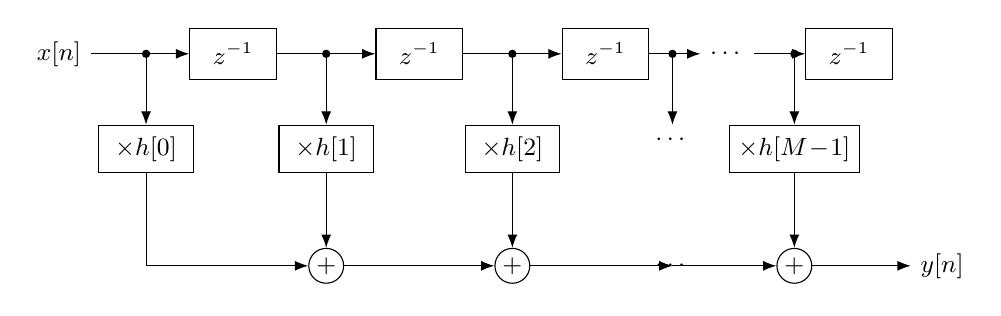
\begin{tikzpicture}[
  >=Latex,
  node distance=1.25cm,
  every node/.style={font=\small}
]
  % --- main delay line
  \node (x) {$x[n]$};
  \node[draw,minimum width=1.1cm,minimum height=0.65cm,right=of x] (z1) {$z^{-1}$};
  \node[draw,minimum width=1.1cm,minimum height=0.65cm,right=of z1] (z2) {$z^{-1}$};
  \node[draw,minimum width=1.1cm,minimum height=0.65cm,right=of z2] (z3) {$z^{-1}$};
  \node[right=0.65cm of z3] (dots) {$\cdots$};
  \node[draw,minimum width=1.1cm,minimum height=0.65cm,right=0.65cm of dots] (zM) {$z^{-1}$};

  \draw[->] (x) -- (z1);
  \draw[->] (z1) -- (z2);
  \draw[->] (z2) -- (z3);
  \draw[->] (z3) -- (dots);
  \draw[->] (dots) -- (zM);

  % tap points (black dots)
  \coordinate (t0) at ($(x)!0.5!(z1)$);
  \coordinate (t1) at ($(z1)!0.5!(z2)$);
  \coordinate (t2) at ($(z2)!0.5!(z3)$);
  \coordinate (t3) at ($(z3)!0.55!(dots)$);
  \coordinate (tM) at ($(dots)!0.55!(zM)$);
  \foreach \p in {t0,t1,t2,t3,tM} {\fill (\p) circle (1.5pt);}

  % multipliers under taps
  \node[draw,minimum width=1.2cm,minimum height=0.6cm,below=0.9cm of t0] (m0) {$\times h[0]$};
  \node[draw,minimum width=1.2cm,minimum height=0.6cm,below=0.9cm of t1] (m1) {$\times h[1]$};
  \node[draw,minimum width=1.2cm,minimum height=0.6cm,below=0.9cm of t2] (m2) {$\times h[2]$};
  \node[below=0.9cm of t3] (mdots) {$\cdots$};
  \node[draw,minimum width=1.25cm,minimum height=0.6cm,below=0.9cm of tM] (mM) {$\times h[M\!- \!1]$};

  \draw[->] (t0) -- (m0);
  \draw[->] (t1) -- (m1);
  \draw[->] (t2) -- (m2);
  \draw[->] (t3) -- (mdots);
  \draw[->] (tM) -- (mM);

  % --- FIXED ADDER CHAIN ---
  % We position adders directly below their corresponding multipliers to ensure alignment
  
  \node[circle,draw,inner sep=1.1pt,below=0.95cm of m1] (a1) {$+$};
  \node[circle,draw,inner sep=1.1pt,below=0.95cm of m2] (a2) {$+$};
  
  % For the dots in the adder line, we position relative to the multiplier dots
  \coordinate (adots) at (mdots |- a1); 
  \node at (adots) {$\cdots$};
  
  \node[circle,draw,inner sep=1.1pt,below=0.95cm of mM] (aM) {$+$};
  \node[right=of aM] (y) {$y[n]$};

  % Connections
  \draw[->] (m0) |- (a1);    % Side entry (Left->Right)
  \draw[->] (m1) -- (a1);    % Top entry (Down)
  \draw[->] (a1) -- (a2);    % Summation flow (Right)
  \draw[->] (m2) -- (a2);    % Top entry (Down)
  \draw[->] (a2) -- (adots); % Summation flow (Right)
  \draw[->] (adots) -- (aM); % Summation flow (Right)
  \draw[->] (mM) -- (aM);    % Top entry (Down)
  \draw[->] (aM) -- (y);     % Output flow (Right)

\end{tikzpicture}

\vspace{0.3em}
{\footnotesize Each tap is a delayed copy $x[n-k]$, scaled by $h[k]$, then summed.}
\end{frame}

%%%%%%%%%%%%%%%%%%%%%%%%%%%%%%%%%
% --- Fourier ---
%%%%%%%%%%%%%%%%%%%%%%%%%%%%%%%%%



\begin{frame}[plain]
    \centering
    \vfill
    {\usebeamerfont{section title}Fourier transform \par}
    \vfill
  \end{frame}

\subsection{Fourier transform (frequency-domain view)}

\begin{frame}{Why go to the frequency domain?}
\small
The Fourier transform decomposes a signal into \textbf{sinusoidal components} (``what frequencies are present?'').

\begin{itemize}
  \item Many physiological phenomena are naturally described by \textbf{bands} (slow vs. fast oscillations).
  \item Noise/artifacts often occupy \textbf{distinct frequency ranges} (e.g., baseline wander vs. muscle noise).
  \item In ML pipelines, spectral features are often more robust than raw samples.
\end{itemize}

\begin{block}{Healthcare examples (Data Science perspective)}
\begin{itemize}
  \item \textbf{ECG:} heart rate and QRS-related energy; remove baseline wander with a high-pass.
  \item \textbf{EEG:} band power (delta/theta/alpha/beta/gamma) as biomarkers/features.
  \item \textbf{PPG:} pulse-rate peak + harmonics; motion artifacts can dominate higher frequencies.
\end{itemize}
\end{block}
\end{frame}

\begin{frame}{Time duration vs. Fourier representations}
\centering
\small
\setlength{\tabcolsep}{3pt}
\renewcommand{\arraystretch}{1.3}

\resizebox{\textwidth}{!}{%
\begin{tabular}{|c|c|c|}
\hline
\multicolumn{2}{|c|}{\textbf{Time Duration}} & \\
\hline
\textbf{Finite} & \textbf{Infinite} & \\
\hline

% --- ROW 1: DISCRETE TIME ---
% Column 1: DFT
\parbox{0.42\textwidth}{\centering
    \textbf{Discrete FT (DFT)} \\[0.5em]
    $\displaystyle X[k]=\sum_{n=0}^{N-1} x[n]e^{-j2\pi kn/N}$ \\[0.5em]
    $k=0,1,\dots,N-1$
} &
% Column 2: DTFT
\parbox{0.42\textwidth}{\centering
    \textbf{Discrete-Time FT (DTFT)} \\[0.5em]
    $\displaystyle X(e^{j\omega})=\sum_{n=-\infty}^{\infty} x[n]e^{-j\omega n}$ \\[0.5em]
    $\omega\in(-\pi,\pi]$
} &
% Column 3: Label
\parbox{0.08\textwidth}{\centering
    discr.\\ time\\ $n$
}
\\ \hline

% --- ROW 2: CONTINUOUS TIME ---
% Column 1: FS
\parbox{0.42\textwidth}{\centering
    \vspace{0.5em} % distinct spacing
    \textbf{Fourier Series (FS)} \\[0.5em]
    $\displaystyle X[k]=\frac{1}{T}\int_{0}^{T} x(t)e^{-jk\omega_0 t}\,dt$ \\[0.5em]
    $k\in\mathbb{Z}, \quad \omega_0=\tfrac{2\pi}{T}$
    \vspace{0.5em}
} &
% Column 2: FT
\parbox{0.42\textwidth}{\centering
    \vspace{0.5em}
    \textbf{Fourier Transform (FT)} \\[0.5em]
    $\displaystyle X(\omega)=\int_{-\infty}^{\infty} x(t)e^{-j\omega t}\,dt$ \\[0.5em]
    $\omega\in(-\infty,\infty)$
    \vspace{0.5em}
} &
% Column 3: Label
\parbox{0.08\textwidth}{\centering
    cont.\\ time\\ $t$
}
\\ \hline

% --- FOOTER: FREQUENCY DOMAIN ---
discrete freq. $k$ & continuous freq. $\omega$ & \\
\hline
\end{tabular}%
}
\end{frame}

\begin{frame}{Continuous-time Fourier transform (CTFT)}
\small
For a continuous-time signal $x(t)$, the Fourier transform is
\[
X(f) = \int_{-\infty}^{\infty} x(t)\,e^{-j2\pi f t}\,dt,
\qquad
x(t) = \int_{-\infty}^{\infty} X(f)\,e^{j2\pi f t}\,df.
\]

\begin{itemize}
  \item $f$ is in Hz; $X(f)$ is complex (magnitude and phase).
  \item $|X(f)|$ tells \textbf{how much} of each frequency is present.
  \item Phase matters for reconstruction, alignment, and system response.
\end{itemize}

\begin{block}{Engineering intuition}
A sinusoid at frequency $f_0$ creates a \textbf{sharp peak} at $f_0$ in $|X(f)|$.
\end{block}
\end{frame}

\begin{frame}{Discrete-time: DTFT, DFT, and FFT}
\small
When we sample $x(t)$ at rate $f_s$ we get $x[n]=x(nT_s)$ with $T_s=\tfrac{1}{f_s}$.

\vspace{0.3em}
\textbf{DTFT (theoretical):}
\[
X\!\left(e^{j\omega}\right) = \sum_{n=-\infty}^{\infty} x[n] e^{-j\omega n}
\qquad (\text{periodic in }\omega).
\]

\vspace{0.3em}
\textbf{DFT (computable on a finite window of length $N$):}
\[
X[k] = \sum_{n=0}^{N-1} x[n] e^{-j2\pi kn/N},\qquad k=0,\dots,N-1.
\]

\begin{itemize}
  \item The \textbf{FFT} is an algorithm that computes the DFT efficiently.
  \item Frequency resolution: $\Delta f = \tfrac{f_s}{N}$ (bin spacing).
  \item Map bins to Hz (for $0\le k\le \tfrac{N}{2}$): $f_k = \tfrac{k f_s}{N}$.
\end{itemize}
\end{frame}

\begin{frame}{Fourier properties you will use constantly}
\small
\begin{columns}[T,onlytextwidth]
\column{0.58\textwidth}
\begin{itemize}
  \item \textbf{Linearity:} $\mathcal{F}\{a x + b y\}= aX+bY$.
  \item \textbf{Convolution theorem:}
  \[
  (x*h)(t) \leftrightarrow X(f)\,H(f).
  \]
  \item \textbf{Multiplication in time} $\Rightarrow$ \textbf{convolution in frequency} (and vice versa).
\end{itemize}
\column{0.35\textwidth}
\begin{block}{Interpretation for filtering}
Designing a filter is often easiest in frequency:
\begin{itemize}
  \item choose $H(f)$ to pass/attenuate bands,
  \item then implement it as FIR/IIR in time.
\end{itemize}
\end{block}
\end{columns}
\end{frame}




\end{document}